\documentclass{40k}

\usepackage{pdflscape}
\usepackage[pdftex,hidelinks]{hyperref}

%%-- For cards
\pgfmathsetmacro{\cardroundingradius}{2mm}
\pgfmathsetmacro{\striproundingradius}{1mm}
\pgfmathsetmacro{\ruleheight}{0.1}
\pgfmathsetmacro{\stripwidth}{1.1}
\pgfmathsetmacro{\stripheight}{1.1}
\pgfmathsetmacro{\strippadding}{0.1}
\pgfmathsetmacro{\textpadding}{0.3}
\newcommand{\stripcolor}{black}
%%-------

\newcommand{\legacytitle}{CAMPAIGN LEGACY}
\newcommand{\legacystory}{Your must accomplish your quest!}
\newcommand{\legacymissiona}{Any}%
\newcommand{\legacyrolea}{Either}%
\newcommand{\legacymissionb}{Any}%
\newcommand{\legacyroleb}{Either}%
\newcommand{\legacymissionc}{Any}%
\newcommand{\legacyrolec}{Either}%
\newcommand{\legacygoal}{CRUSH FACE.}%
\newcommand{\legacybonus}{Hit yourself.}%

\pgfmathsetmacro{\legacycardwidth}{9.25}
\pgfmathsetmacro{\legacycardheight}{11.85}

\newcommand{\legacystripfontsize}{\Large}
\newcommand{\legacytextfontsize}{\small}

\newcommand{\legacystriptext}%
  {LEGACY: \legacytitle\hspace{0.5em}\rotatebox[origin=c]{-90}{\includegraphics[width=0.6cm]{icon-skull}}}


%%----------------------------------------------------------------------
%%----------------------------------------------------------------------
\newcommand{\resultstable}{%
\noindent\begin{minipage}{\linewidth}%
%\smallskip\centering\legacytextfontsize%
{\bf Recon Squad Missions:}\\
\centerline{\begin{tabular}{@{}C{1.3in}C{1in}c@{}}
  %{\bf Mission} & {\bf Role}&\\% & {\bf Victory}\\
  %\hline
  \legacymissiona & \legacyrolea & \ding{111}\\
  \legacymissionb & \legacyroleb & \ding{111}\\
  \legacymissionc & \legacyrolec & \ding{111}\\
  %\underline{\hspace{1.25in}} &  \underline{\hspace{0.8in}} & \ding{111}\\
\end{tabular}}%
\end{minipage}%
}


%%----------------------------------------------------------------------
%%----------------------------------------------------------------------
\newcommand{\drawlegacycard}{%
\begin{tikzpicture}%
  \clip (-0.05, -0.05) rectangle (\legacycardwidth+.05, \legacycardheight+.05);

  %%-- Draw the card back and outline
  \draw[rounded corners=\cardroundingradius,fill=white,draw=none] (0,0)
    rectangle (\legacycardwidth,\legacycardheight);
  \node[above left] at (\legacycardwidth+0.1, -0.1)
    {\includegraphics[width=3.5in]{background-skull}};
  \draw[rounded corners=\cardroundingradius] (0,0) rectangle
    (\legacycardwidth,\legacycardheight);

  %%-- Draw the side strip
  \fill[\stripcolor,rounded corners=\striproundingradius]
    (\strippadding,\strippadding) rectangle
    (\strippadding+\stripwidth,\legacycardheight-\strippadding)
    node[rotate=90,above left,white,font=\legacystripfontsize\fontfamily{ptm}\selectfont] {\raisebox{0pt}[12pt][4pt]{\vbox to -18pt{}} \legacystriptext};

  %%-- Draw the player info lines
    \node[text width=(\legacycardwidth-\strippadding-\stripwidth-2*\textpadding)*1cm,
          below right,inner sep=0] at
          (\strippadding+\stripwidth+\textpadding,\legacycardheight-\textpadding)
    {\legacytextfontsize%
      \raisebox{0pt}[26pt][0pt]{\begin{minipage}[b]{1.0\linewidth}\centering\it
          \legacystory
      \end{minipage}}

      %\bigskip
      %\centerline{\Large\sc\fontfamily{ptm}\selectfont --- Campaign ---}

      \bigskip
      \centerline{\resultstable}

      %\bigskip
      %\centerline{\Large\sc\fontfamily{ptm}\selectfont --- Cataclysm ---}

      \bigskip
      {\bf Cataclysm Objective:} \legacygoal

      \bigskip
      {\bf Legacy Bonus:} \legacybonus
    };

    \node[text width=(\legacycardwidth-\strippadding-\stripwidth-2*\textpadding)*1cm,
          above right,inner sep=0] at
          (\strippadding+\stripwidth+\textpadding,\strippadding)
    {\legacytextfontsize%
      \begin{tabular}{@{}ll}
        \textbf{Name:} &  \underline{\vbox to 18pt{}\hspace{2.125in}}\\
        %\textbf{Squad:} &  \underline{\vbox to 18pt{}\hspace{8.25cm}}\\
        %\textbf{Faction:} & \underline{\vbox to 18pt{}\hspace{8.25cm}}\\
        %\textbf{Alliance:} & \underline{\vbox to 18pt{}\hspace{8.25cm}}\\
      \end{tabular}
    };
\end{tikzpicture}
}


\newcommand{\legacycard}[9]{%
\renewcommand{\legacytitle}{#1}%
\renewcommand{\legacystory}{#2}%
\renewcommand{\legacymissiona}{#3}%
\renewcommand{\legacyrolea}{#4}%
\renewcommand{\legacymissionb}{#5}%
\renewcommand{\legacyroleb}{#6}%
\renewcommand{\legacymissionc}{#7}%
\renewcommand{\legacyrolec}{#8}%
\renewcommand{\legacygoal}{#9}%
\legacycardb%
}

\newcommand{\legacycardb}[1]{%
\renewcommand{\legacybonus}{#1}%
\drawlegacycard%
}


\begin{document}

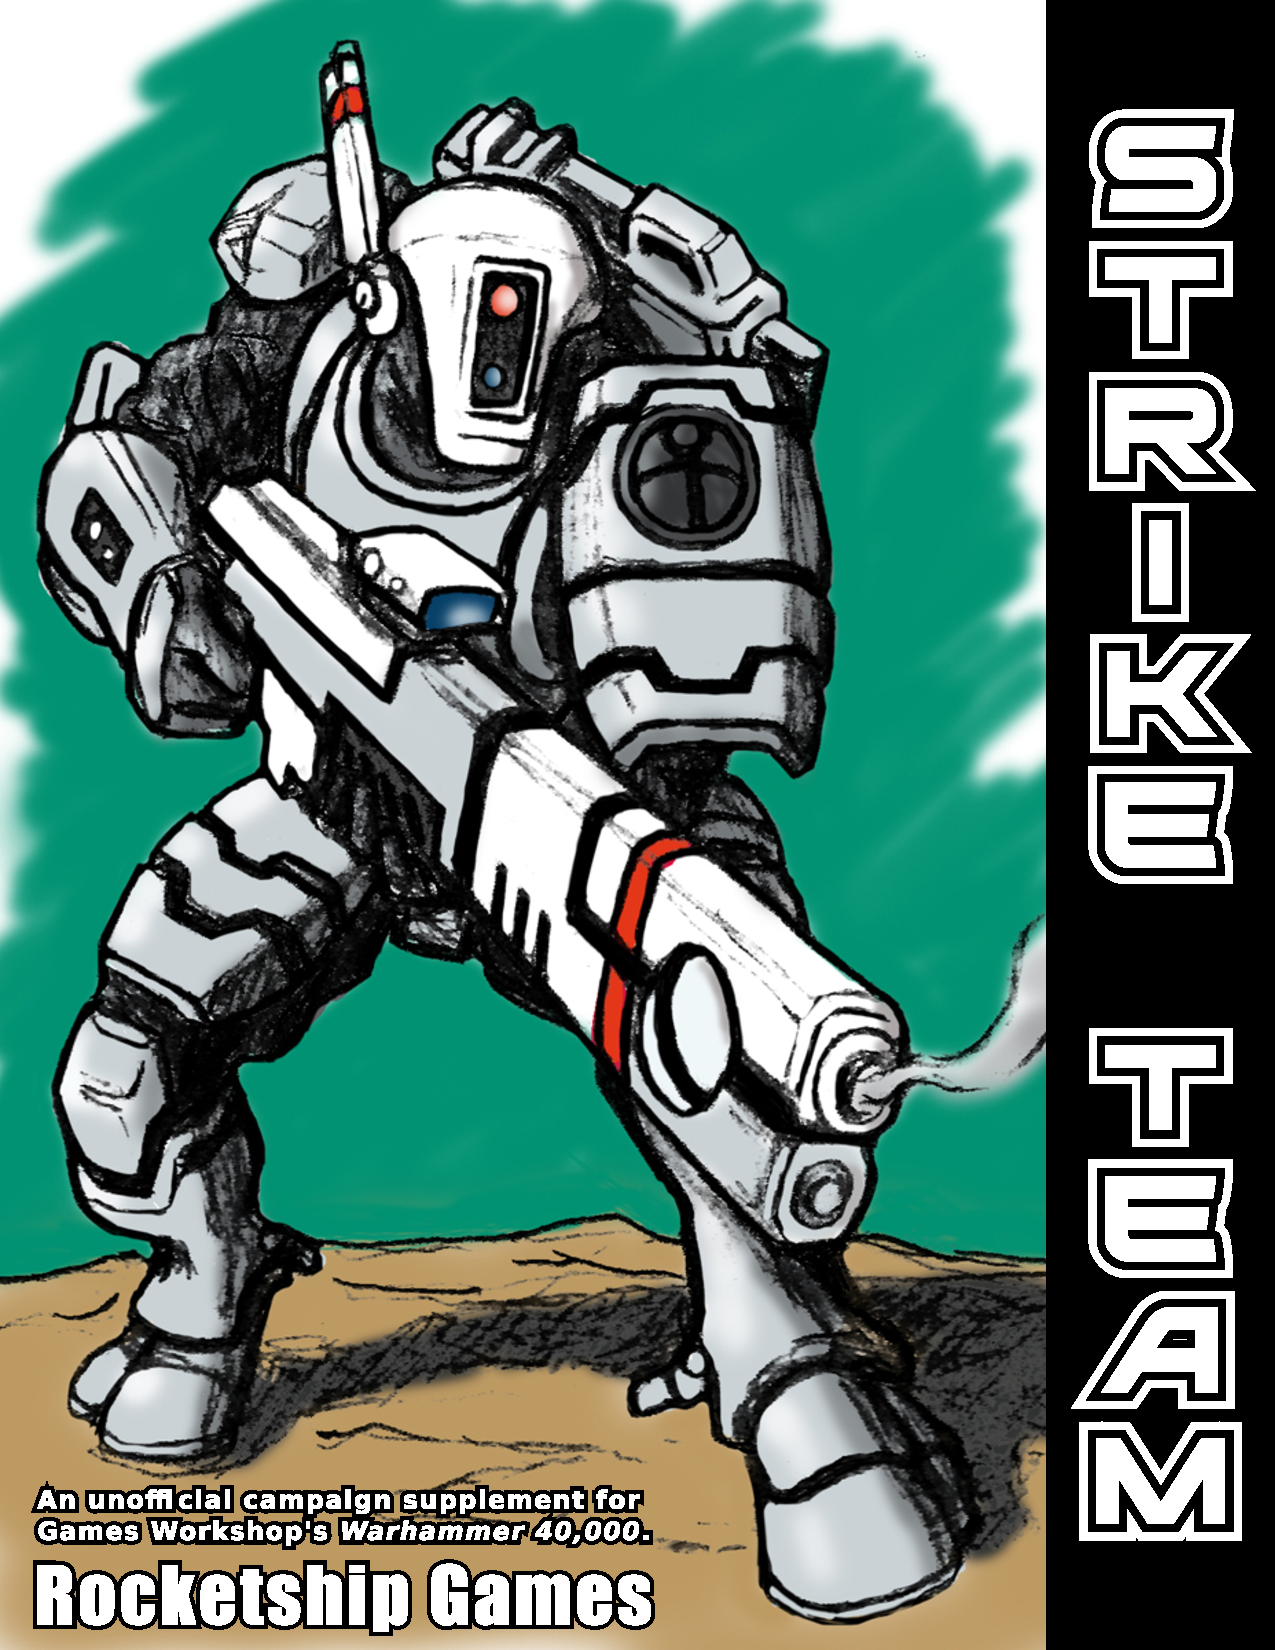
\includepdf[pages={1}]{art/cover/cover.pdf}

%%----------------------------------------------------------------------
%%----------------------------------------------------------------------
\section{Introduction}

\begin{columns}

  \emph{Legacies} is an unofficial, team-oriented skirmish campaign
  for Games Workshop's \emph{Warhammer 40,000}.  Its core is a set of
  eight thematic missions designed for \emph{Recon Squad}, an
  unofficial skirmish variant of \emph{40k} similar to Games
  Workshop's \emph{Kill Team} rules.  Players field only a squad or
  two on a small board with dense terrain, and all their models act
  independently.  It's a very different \emph{40k} experience, focused
  on the heroics of regular grunts, without requiring you to learn new
  core rules.

  Those skirmishes are woven into a campaign here by a set of eight
  Legacies, specific missions the recon squads are striving to
  complete for their alliance.  The campaign climaxes in the
  Cataclysm, in which all the recon squads and some reinforcements
  fight alongside their alliance teammates in a final joint battle.

  \emph{Legacies} may be run either as a single full-day event or over
  several evenings.  Though the missions and legacies are thematic and
  storyful, \emph{Legacies} does not have its own setting, so that it
  can be easily adapted to one of your own making.  Other events are
  also easily connected before or after this campaign to form a larger
  narrative.  Notes are also included here on scoring \emph{Legacies}
  in a narrative tournament or league with individual prizes.

  Recon Squad rules are available here:

  \centerline{\url{rocketshipgames.com/40k/recon-squad/}}

\columnbreak
\noindent\fbox{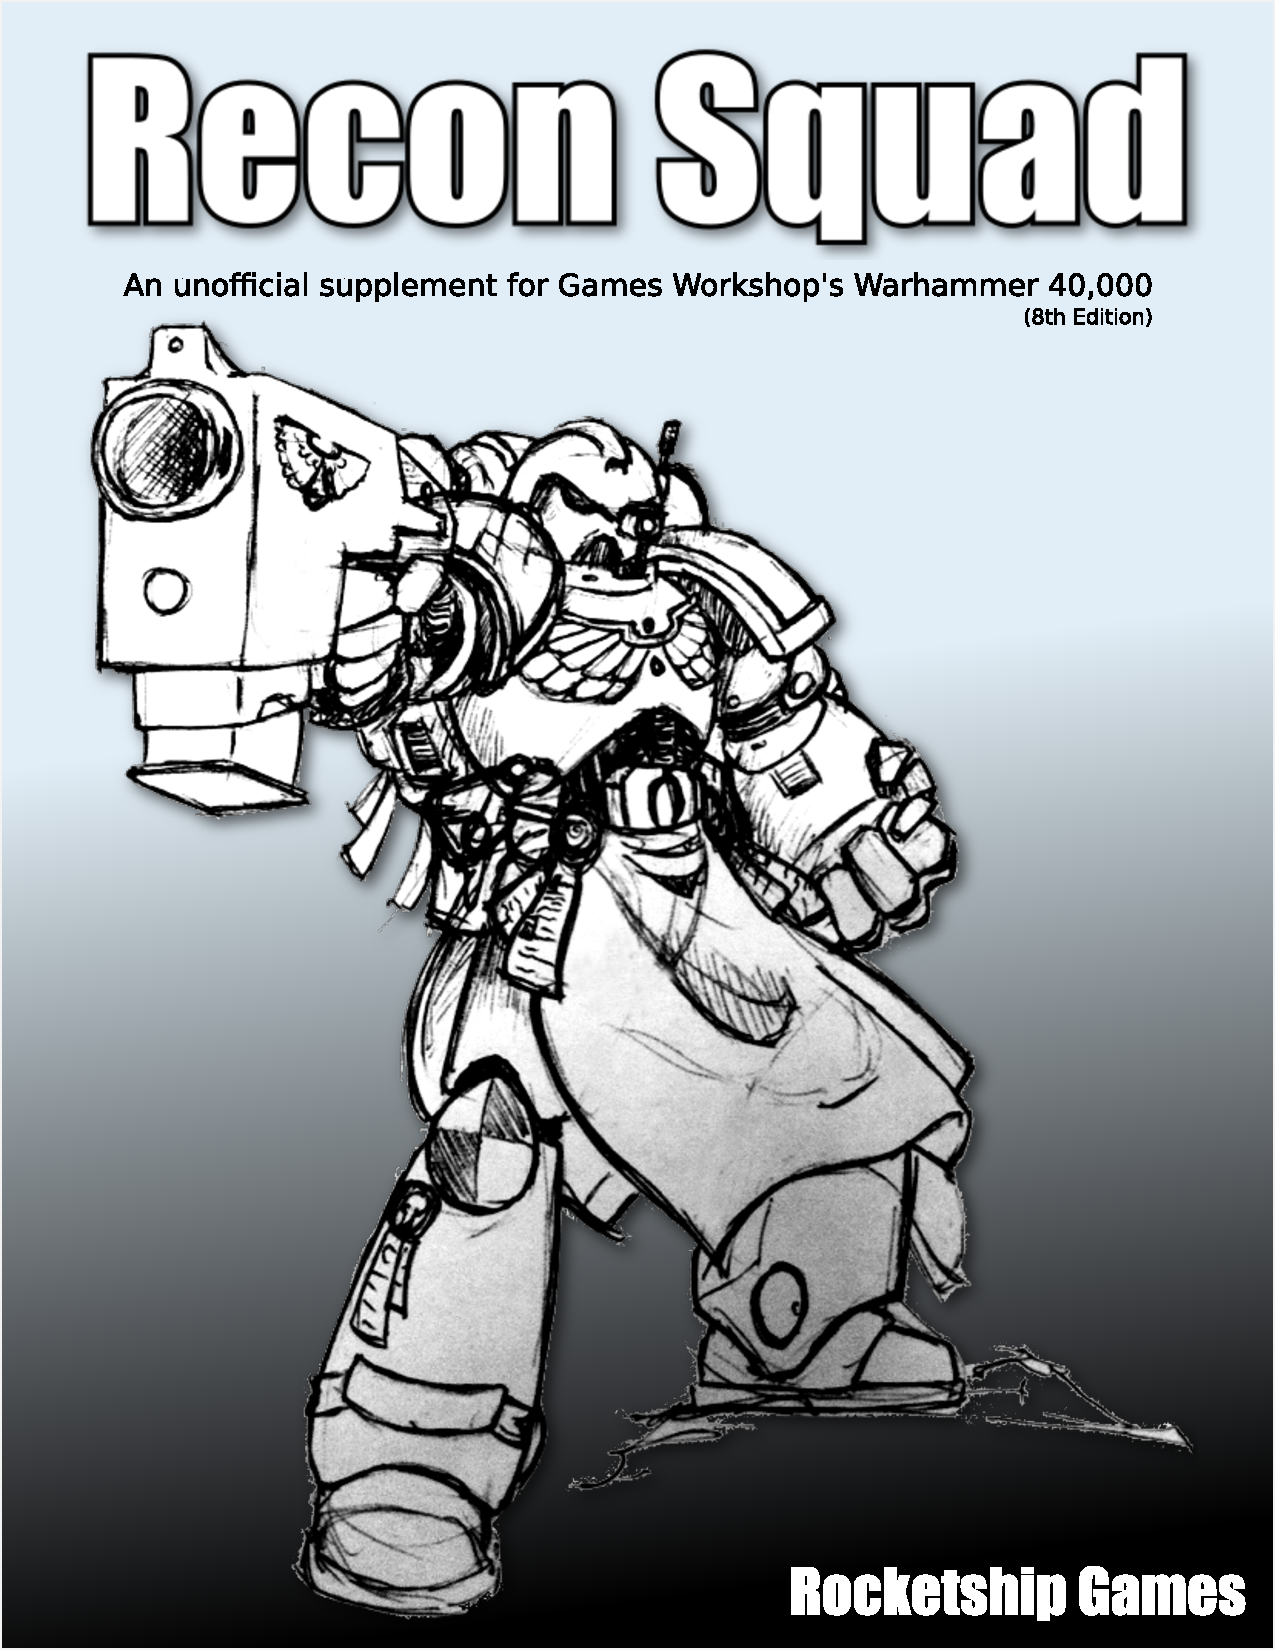
\includegraphics[width=\linewidth]{art/recon-squad_cover.pdf}}
  
\subsection{Overview}

\emph{Legacies} is played as four rounds of Recon Squad skirmishes,
capturing small but pivotal incidents in a larger battle, followed by
a closing Cataclysm team game.

Each player's squad is working toward a legacy within the
greater conflict---

\begin{squishitemize}
\item \textbf{Bodyguards:} Fierce defenders of battlefield
  commanders;

\item \textbf{Excavators:} Daring explorers, technical experts, and
  artifact raiders;

\item \textbf{Headhunters:} Precision instruments of
  targeted violence;
%\end{squishitemize}

  % Following the events of \emph{The Debacle on Caldor IV} it has
  % become clear that the legendary \emph{Scythe of Unbound Light}
  % exists and is immeasurably important.  This discovery has spun the
  % maelstrom of conflict on Caldor IV to even dizzier velocities.
  % Unfortunately, the destruction of the planet is also now inevitable
  % with the Imperium having begun Exterminatus.  With every army
  % shattered and communication all but impossible, it is up to the
  % individual commanders and warriors in the field to rise to the
  % moment.  \emph{The Twilight of Caldor IV} plots the heroics of small
  % bands of warriors furiously moving into position to help their
  % alliance claim the relic before the end.


%\begin{squishitemize}
\item \textbf{Killers:} Shattered fighters disconnected from anything
  but bloodshed;

\item \textbf{Penetrators:} Sharpened blades able to break any
  armor or defense;

\item \textbf{Scouts:} Reckless adventurers reconnoitering the
  battlefield;

\item \textbf{Sentinels:} Implacable defenders and masters of \emph{ad
    hoc} fortifications;

\item \textbf{Warriors:} Hardened veterans that have been through
  everything.
\end{squishitemize}

Their path toward those legacies is defined by the missions they
tackle:

\smallskip\centerline{\begin{tabular}{C{1.5in}C{1.5in}}
\textbf{Ambush} & \textbf{Encirclement}\\
\textbf{Assassination} & \textbf{Excavation}\\
\textbf{Battlefield} & \textbf{Installation}\\
\textbf{Breakthrough} & \textbf{Skirmish}\\
\end{tabular}}

\smallskip%
Successes and failures at those challenges will define both the recon
squad's place in history, and their alliance's ability to win out in
the final Cataclysm.

\end{columns}

%%----------------------------------------------------------------------
%%----------------------------------------------------------------------
\clearpage
\pagetitle{Organization}

\begin{columns}

This section describes how to conduct a \emph{Legacies} campaign, and
is mostly intended for the organizer.

\missionheading{Schedule}

Recon Squad games can be easily run in about~60 minutes in an event
setting with boards pre-arranged and armies unpacked before the clock
starts for each round.  Generally matches take at most~90 minutes even
at a very casual pace with no preparation beforehand.  The Cataclysm
game can be comfortably played in~4 hours including setup.  It's
therefore feasible to run \emph{Legacies} over either several
evenings, or a single full day.  A sample schedule for a single-day is:

\bigskip
\centerline{\begin{tabular}{cl}
11:00	 	& Doors open\\
11:50	 	& Registration Closes\\
12:00	 	& Campaign Briefing \& Alliance Pairings\\
12:15	 	& Round 1\\
1:25	 	& Alliance Pairings\\
1:35	 	& Round 2\\
2:40	 	& Alliance Pairings\\
2:50	 	& Round 3\\
3:50	 	& Alliance Pairings\\
4:00	 	& Round 4\\
5:00	 	& Dinner Break\\
5:30	 	& The Cataclysm\\
9:30	 	& Campaign Outcome \& Prizes\\
\end{tabular}}

\vfill

\noindent\fbox{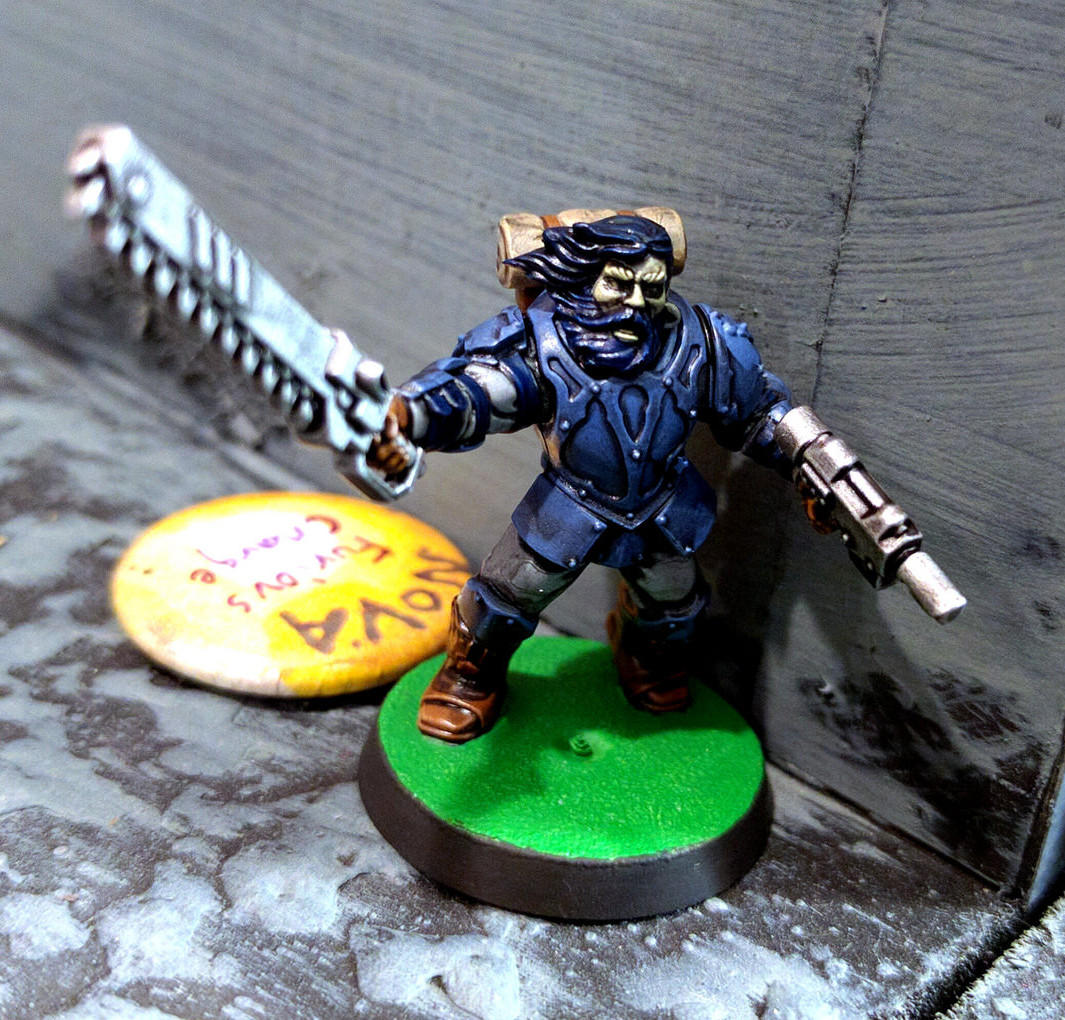
\includegraphics[width=\linewidth]{images/renegade-sgt-cropped.jpg}}

\columnbreak%

\missionheading{Alliances \& Story}

At the start of the campaign, the players are organized into two
alliances with an equal number of players.  In some groups this might
be faction specific, e.g., Chaos Daemons versus Eldar.  Generally
though an alliance will be comprised of several factions and can be
given a less specific title such as the Forces of Order, Legions of
Discord, or the Spoiler Horde.  How players are assigned alliances is
up to the organizer.  In a large event with mostly strangers and
tournament leanings it might be simply random.  In more
narrative-oriented and casual settings though, some attempt should be
made to take into account thematic cohesiveness as well as balanced
skill levels.

The concept behind the campaign is that each recon squad is a team of
veterans or other distinguished warriors tasked with several special
operations as part of a larger battle or war.  In the course of those
missions their paths eventually all cross, resulting in the larger
final battle.  Any specific background story is up to the organizer
and players, enabling a range of narratives with more or less detail.

\missionheading{Setup}

In advance of the campaign, players should be pointed to the Recon
Squad rules and the Missions section of this packet so they can design
their Recon Squad and Cataclysm army lists.  The campaign is themed
around players fielding a single Recon Squad list throughout, but the
organizer should feel free to be flexible about that requirement if
they wish.  In a campaign run over multiple days there is no need to
require Cataclysm lists be finalized until the last event.

Preparing for the campaign is very simple.  For each of the two
alliances, print and cut apart enough sets of the~8 legacy cards in
the Missions section to have at least one card per player.
Also print and cut apart enough sets of the~8 mission sheets to have
one for each match.  For a campaign with up to~16 players this means
making two sets of legacy cards and one set of mission sheets.

With anything but a very small number of players, it's probably easier
to have players record results separately from the mission sheets,
especially as the latter might be used multiple times.  In that case,
print and cut apart enough copies of the scorecards at the end of this
section to have one for each match.  Finally, if using the scoring
mechanism described here, also print and cut apart enough copies of
the ballots and tickets from the end of this section to have one
painting ballot per player and as many sportsmanship tickets as you
think might be necessary.

\missionheading{Legacies}

After being assigned an alliance, each player chooses a legacy.  No
legacy may be selected twice within an alliance until all legacies
have been chosen at least once, and so on if there are even more
players.  Otherwise the alliance members may discuss among themselves
how to divy up the legacies.  If there is any contention, either ask
the players in random order to choose, or randomly assign legacies.

Each legacy lists three Recon Squad Missions and gives a Cataclysm
Objective and Legacy Bonus.  To achieve their legacy, players must
accomplish the Cataclysm Objective in the final team battle.  If they
win at least two of the three Recon Squad Missions in the given role
of attacker, defender, or either, then they receive their Legacy Bonus
in the Cataclysm.

Players' chosen legacies, match results, and whether or not they are
succeeding at their missions are all public information throughout the
campaign.

\missionheading{Round Pairings}

Recon Squad match pairings are made strategically by the alliances to
help their players achieve their legacy missions and further their
collective strategic goals.  Before each round, the alliances
alternate nominating one of their remaining unpaired players along
with a mission and role (attacker or defender).  The opposing alliance
then responds with a player for the match, who takes the other mission
role and chooses an unclaimed game board to play on.  This player must
be in the same or best similar win/draw/loss bracket as the nominated
player, unless the number of players is not great enough to make this
restriction without repeating match pairings.  In that case the later
rounds might require specific pairings to not have repeats.

For the first round, the initial alliance to put a player forward is
determined either randomly or based on the background story or the
outcomes of connected preceding events.  In subsequent rounds the
alliances alternate making the initial nomination.

\columnbreak

Players should use the checkboxes on their legacy cards to record
victories toward the Recon Squad Mission requirements, in addition to
the organizer keeping track.  It does not matter if the player was
nominated or the responding opponent, and they do not have to complete
the missions in any order.  In order to get their Legacy Bonus in the
Cataclysm they simply have to win each mission in the required role at
some point in the campaign.  Similarly, a player can attempt a mission
and role pair multiple times.  However, no advantage is gained by
winning the same mission and role pair multiple times.

\missionheading{Cataclysm}

Following the four rounds of Recon Squad games, the campaign concludes
by pitching the two teams against each other directly in the
Cataclysm.  Each player essentially adds 300 points to their Recon
Squad, as described in detail in the Missions section.


\missionsubheading{Board.}  The table for the Cataclysm game should be~4'
wide as usual, and roughly as many feet long as there are players in
the campaign.  So an~8-player campaign would conclude on an 8'x4'
table.  One idea to consider is simply moving together boards used in
the Recon Squad rounds, so that the battle thematically continues
directly over the same terrain.

\missionsubheading{Schedule.} The Cataclysm runs for a fixed 5 turns.
The organizer should determine and then enforce a schedule within the
time allotted for the match to ensure it completes, setting a specific
number of minutes for each turn.  Remember that later turns tend to go
faster as models have been removed.  A reasonable schedule of alliance
turns for a~4 hour period, accommodating setup, teardown, and scoring,
is:

\bigskip
\centerline{\begin{tabular}{cc}
Deployment & 15 minutes each\\
Turn 1& 20 minutes each\\
Turn 2& 20 minutes each\\
Turn 3& 15 minutes each\\
Turn 4& 15 minutes each\\
Turn 5& 10 minutes each\\
\end{tabular}}

\bigskip%
It is also important to ensure that enough time is reserved within
each alliance's turn to resolve the assault phase.  Players and armies
focused on close combat might otherwise be disadvantaged.  The
organizer should make sure alliances move on to the assault phase with
time to resolve combats as necessary, even if it means cutting short
their other actions.


%An important role for the organizer in the Cataclysm is keeping time.
%A schedule must be established

\missionheading{Scoring and Prizes}

\emph{Legacies} is oriented to casual play but can easily be used for
a narrative tournament.  Prizes should be kept small and well
distributed though to limit the stakes, given that top players may not
face each other if they're in the same alliance, players don't all
contest the same scenarios, some missions are asymmetric, and so on.
There should also perhaps be two sets of prizes for any gameplay
awards, one for each alliance.  This section outlines one possible
narrative tournament scoring and prize scheme.

\missionsubheading{Prizes.} The following prizes are offered:

\begin{itemize}\shortlist
\item Winners in each alliance by overall scores;
\item Painting award based on player voting;
\item Best squad leader by top game results.
\end{itemize}

\missionsubheading{Overall Scores.} A total of~100 points are
available for each player throughout the campaign:

\begin{itemize}\shortlist
\item 60 points for game results;
\item 20 points for painting and craftsmanship;
\item 20 points for sportsmanship.
\end{itemize}

\missionsubheading{Game Results.} 

Each of the four Recon Squad missions are worth up to~12 points.
Major victories award~10 points to the winner and 0 to the not-winner.
Minor victories award~7 points to the winner and 3 to the not-winner.
Draws award~5 points to both players.  Each mission has~2 bonus points
available.

% \begin{itemize}\shortlist
% \item Major victories award~10 points to the winner and 0 to the not-winner;
%\item Minor victories award~7 points to the winner and 3 to the not-winner;
%\item Draws award~5 points to both players.
%\item 2 bonus points are available in each mission.
%\end{itemize}

Players may also earn up to~12 points in the Cataclysm toward their
individual game results:
\begin{itemize}\shortlist
\item 7 points for winning their Cataclysm Objective;
\item 3 points if they earned their Legacy Bonus;
\item 2 points if their alliance won the Cataclysm.
\end{itemize}


\missionsubheading{Painting and Craftsmanship.} 

Painting and craft work is scored objectively by the organizer
applying this rubric to the entire army:

\begin{itemize}\shortlist
\item All models assembled and primed: \hfill +5 pts
\item All models three-color minimum: \hfill +5 pts
\item All models based (paint/flock): \hfill +4 pts
\item Advanced painting techniques present on any model (washes,
  drybrushing, etc.): \hfill +3 pts
\item Advanced basing techniques present on any model (3D details,
  varied flock, etc.): \hfill +3 pts
\end{itemize}

Note that this goes solely toward overall scores.  The painting award
is based purely on player voting.

\columnbreak

%\noindent\fbox{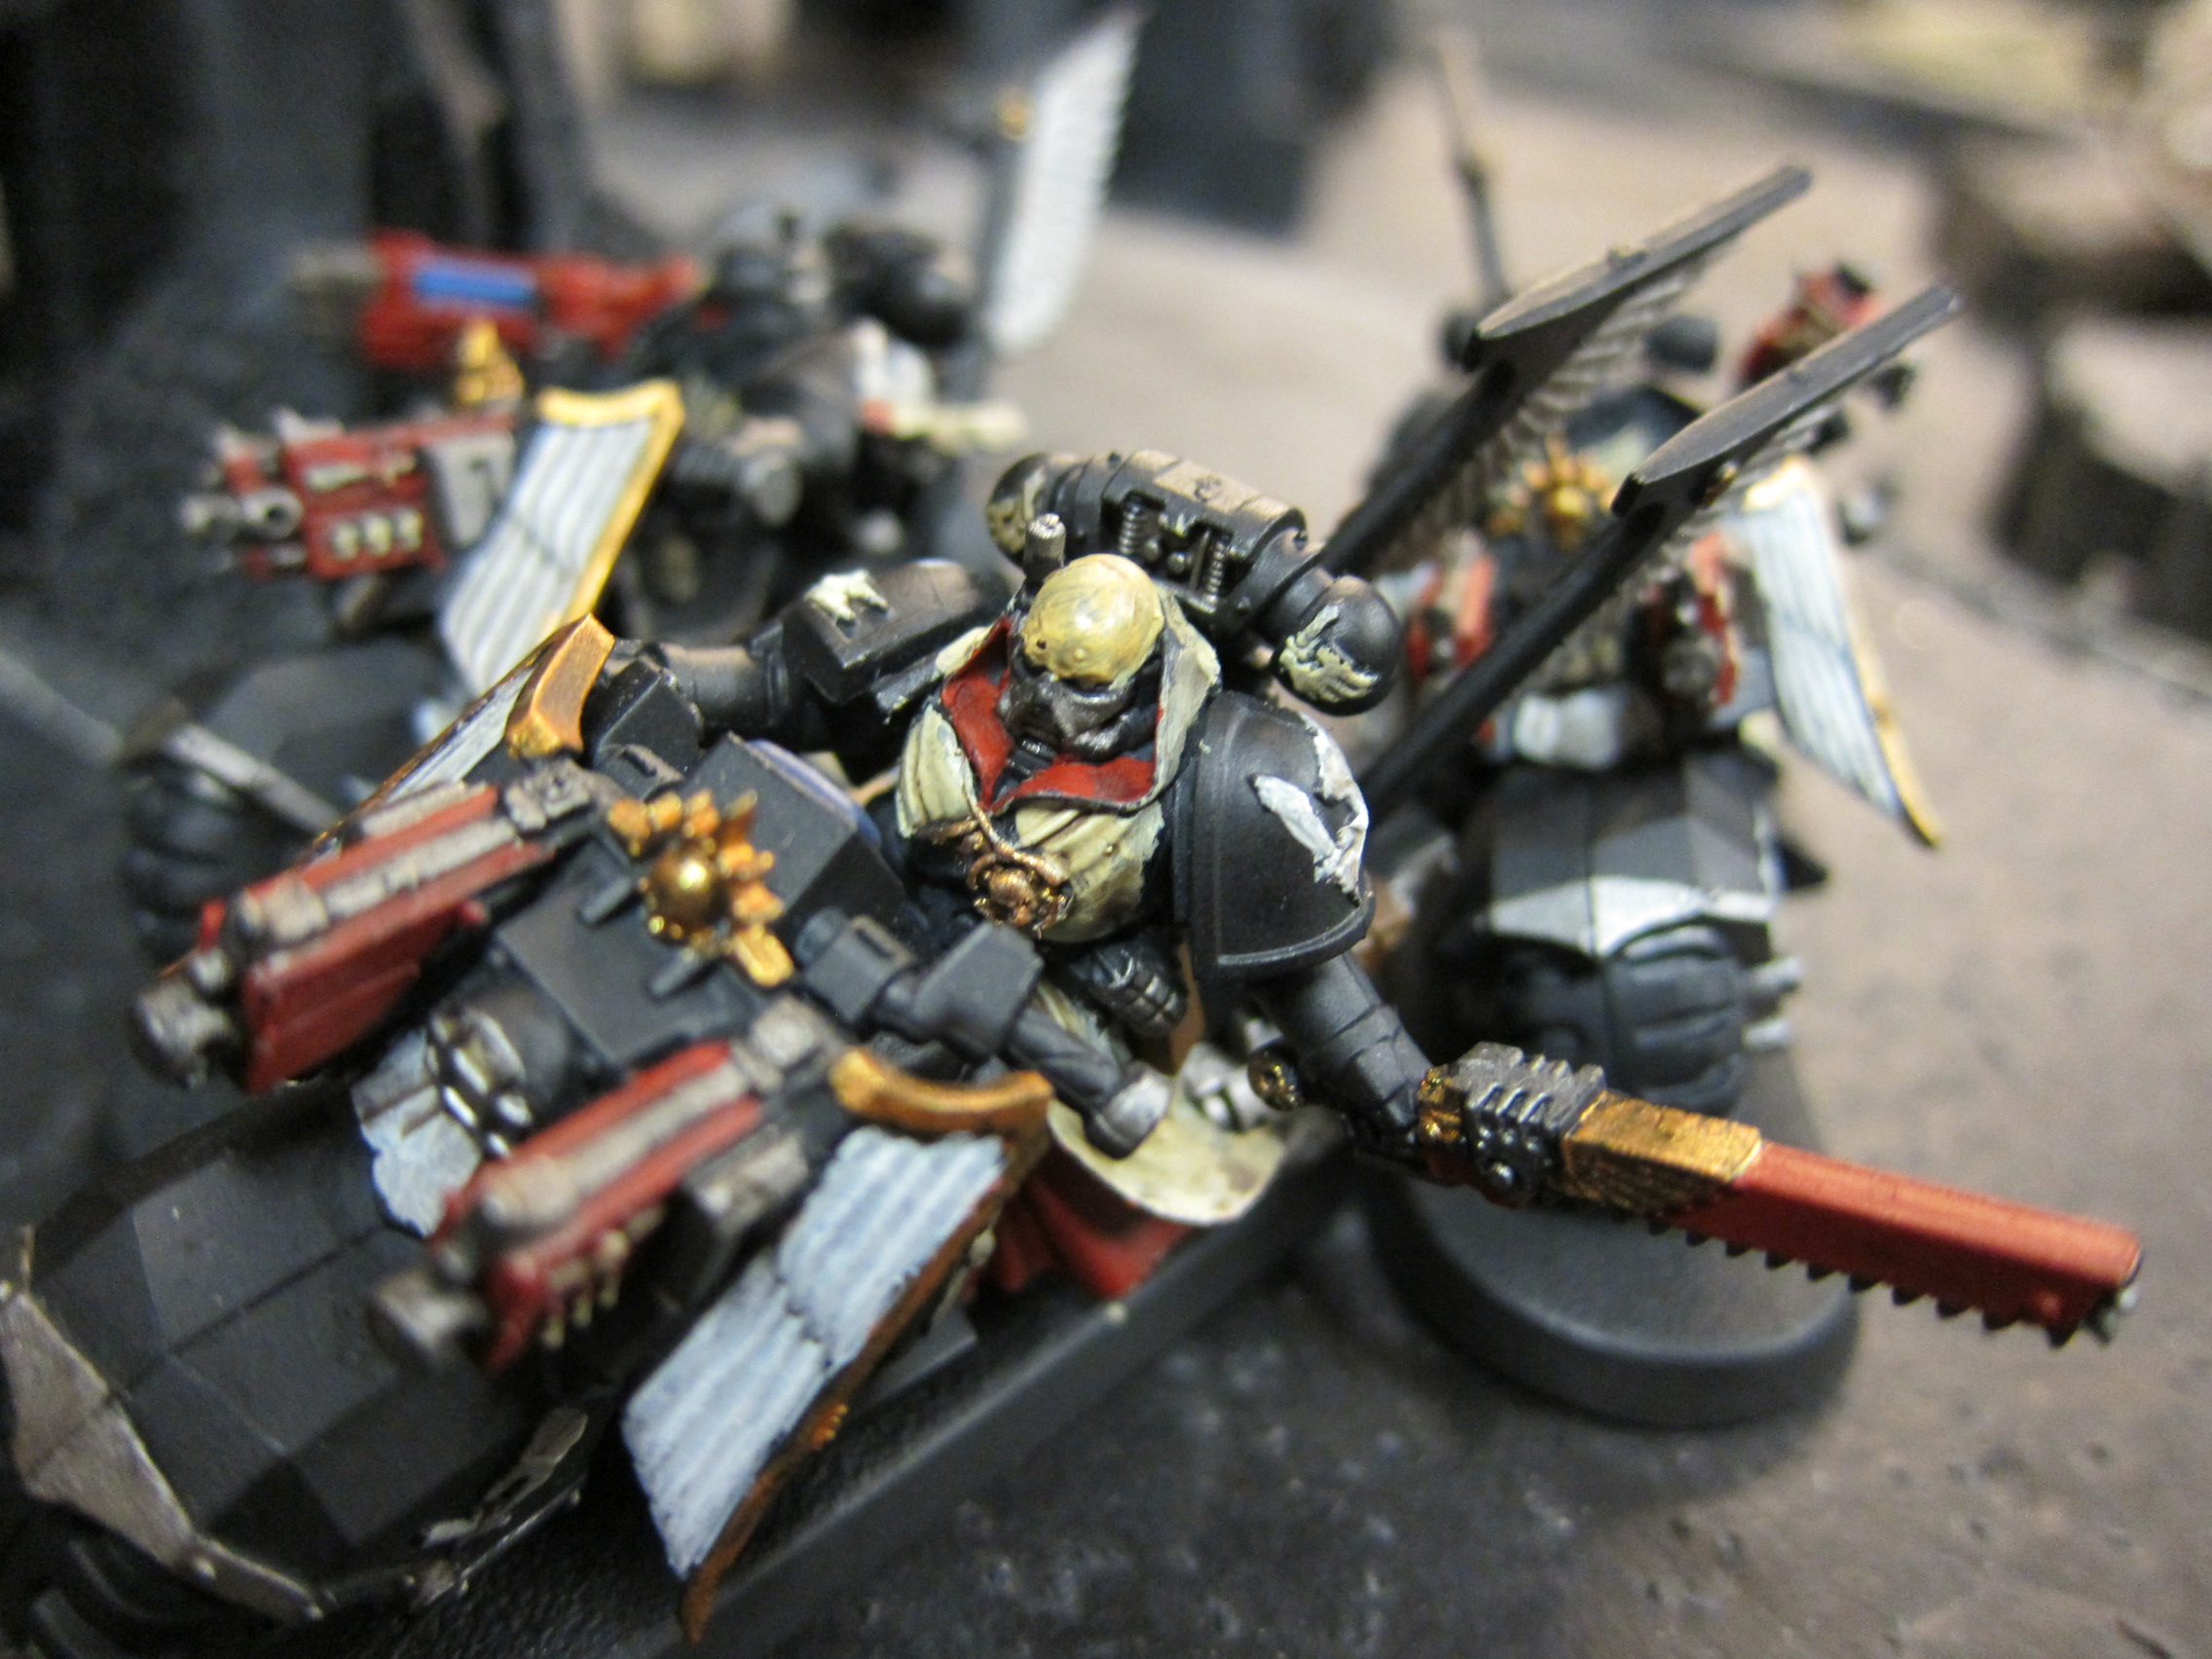
\includegraphics[width=\linewidth]{images/biker-sergeant}}\\
\noindent\fbox{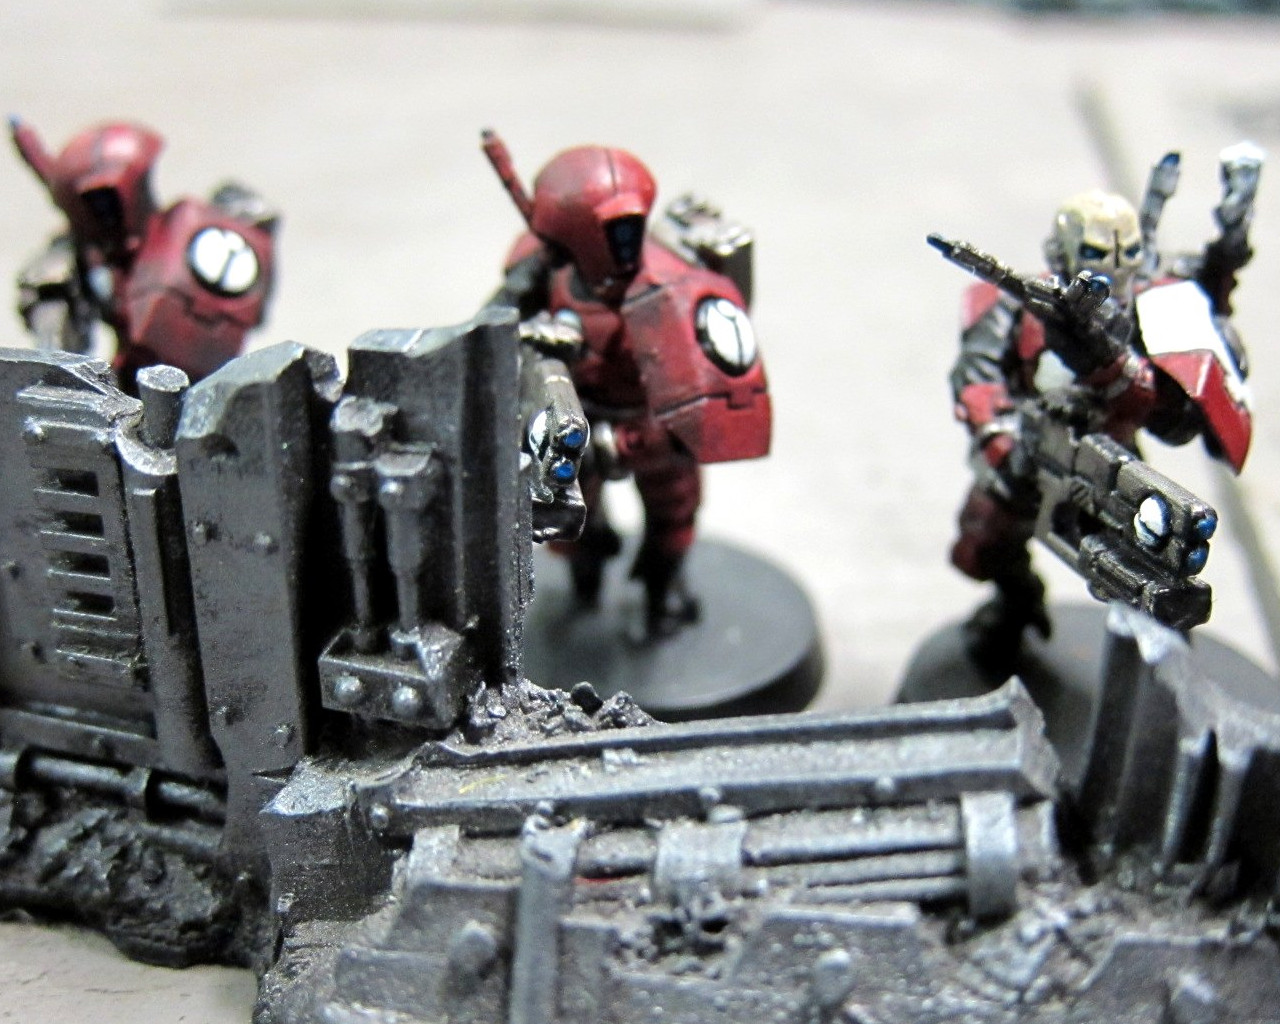
\includegraphics[width=\linewidth]{images/tau-line-cropped}}\\

%\vspace{12pt}
%\noindent\raisebox{0pt}[0.75in]{%
%\begin{minipage}{1.0\linewidth}  
\begin{story}{0.75in}{The Greater Good}
  Shas'ui Ke'ssai crouched behind the crude rubble barricade.  His
  hooves trembled with the clamorous approach of the humans' ugly,
  stinking, smoking vehicles.  In that moment, he realized he hated
  them.  He hated them for their violence, and he hated them for what
  they'd done to his world.  But most of all, he hated them for
  teaching him to hate.
\end{story}%
%\end{minipage}
%}

%\vspace*{-4pt}

%\vspace*{-4pt}
\missionsubheading{Sportsmanship.}

By default players earn~5 points for sportsmanship in each Recon Squad
round.  However, they may be docked points for poor behavior by an
opponent submitting a sportsmanship ticket:

\vspace*{-18pt}
\begin{itemize}\shortlist\setlength{\parskip}{0pt}\setlength{\itemsep}{2pt}
\item Openly hostile or rude: \hfill -3 pts
\item Unnecessarily competitive: \hfill -2 pts
\item Sloppy measuring, line of sight, or dice: \hfill -2 pts
\item Unreasonably late, slow, or inattentive: \hfill -1 pt
\item Significantly unfamiliar with rules:
  \hfill -1 pt
\item Not prepared with clear, typed army lists: \hfill -1 pt
\end{itemize}

\vspace*{-18pt}
Hopefully few or no tickets need be submitted; it's perfectly
acceptable for players to not penalize opponents.  It should be
feasible to supply each player one ticket to start and only give out
more as needed.

\missionsubheading{Painting Award.}  The painting award is determined
by player voting, not the painting scores.  Each player must submit a
ballot of what they consider the top three best-made armies, excluding
themselves, awarding~3,~2, and~1 votes.  The most votes wins.

%\vfill\vbox to 0pt{}
\end{columns}

\squelchbackground
\newcommand{\scorecard}{%
\begin{minipage}{3.25in}\centering
\begin{story}{62pt}{Game Results}
%\vspace*{2pt}

\vspace*{6pt}
{Attacker:}\raisebox{-4pt}{\hbox to 2.0625in{\enspace\hrulefill}}

\vspace*{8pt}
{Defender:}\raisebox{-4pt}{\hbox to 2in{\enspace\hrulefill}}

\vspace*{4pt}
\centering
\begin{minipage}{\linewidth}
{\vbox{\small%
\setlength{\tabcolsep}{2pt}%
\noindent\begin{tabularx}{\linewidth}{cccX}
  \raisebox{6pt}{\hbox to 1.25em{\rotatebox{15}{\small\bf Attacker}}}&
  \hbox to 1.25em{\rotatebox{15}{\small\bf Defender}}&
  &
  \multicolumn{1}{c}{\footnotesize\bf Outcome}
\\
  \hline
%
  \rescheck&\rescheck& & {\bf Major Victory}\\
%
  \rescheck&\rescheck& &
  {\bf Minor Victory}\\
%
\rescheck&\rescheck& &
{\bf Draw}\\
\hline \rescheck&\rescheck& &
{\bf Bonus Point}\\
\rescheck&\rescheck& &
{\bf Bonus Point}\\
\end{tabularx}%
}}%
\end{minipage}

\vspace*{9pt}
\vbox to 0pt{}

\end{story}
\end{minipage}
}

\clearpage
\begin{landscape}  
\noindent
\scorecard%
\hfill%
\scorecard%
\hfill%
\scorecard

\vfill

\noindent
\scorecard%
\hfill%
\scorecard%
\hfill%
\scorecard

\vfill

\noindent
\scorecard%
\hfill%
\scorecard%
\hfill%
\scorecard

\end{landscape}
\clearpage

%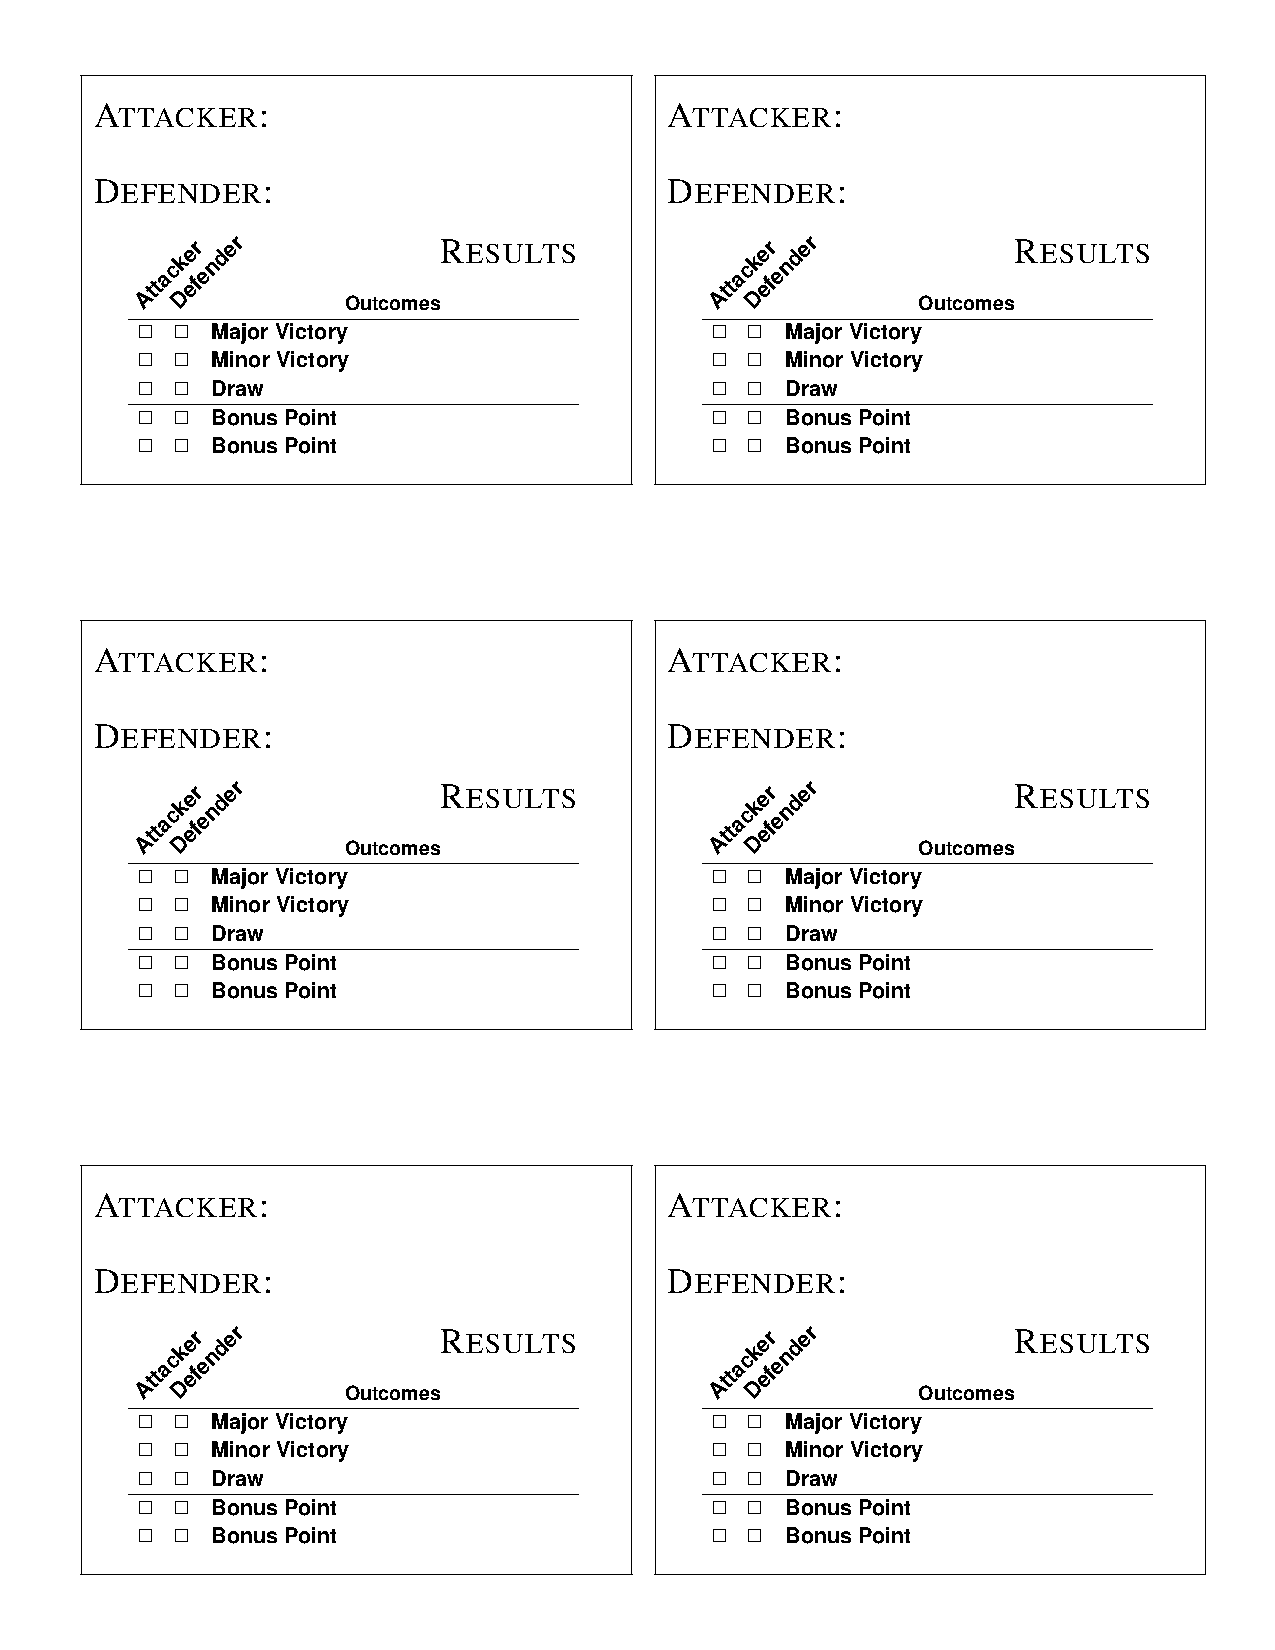
\includepdf[pages={1}]{20141220-scorecards.pdf}
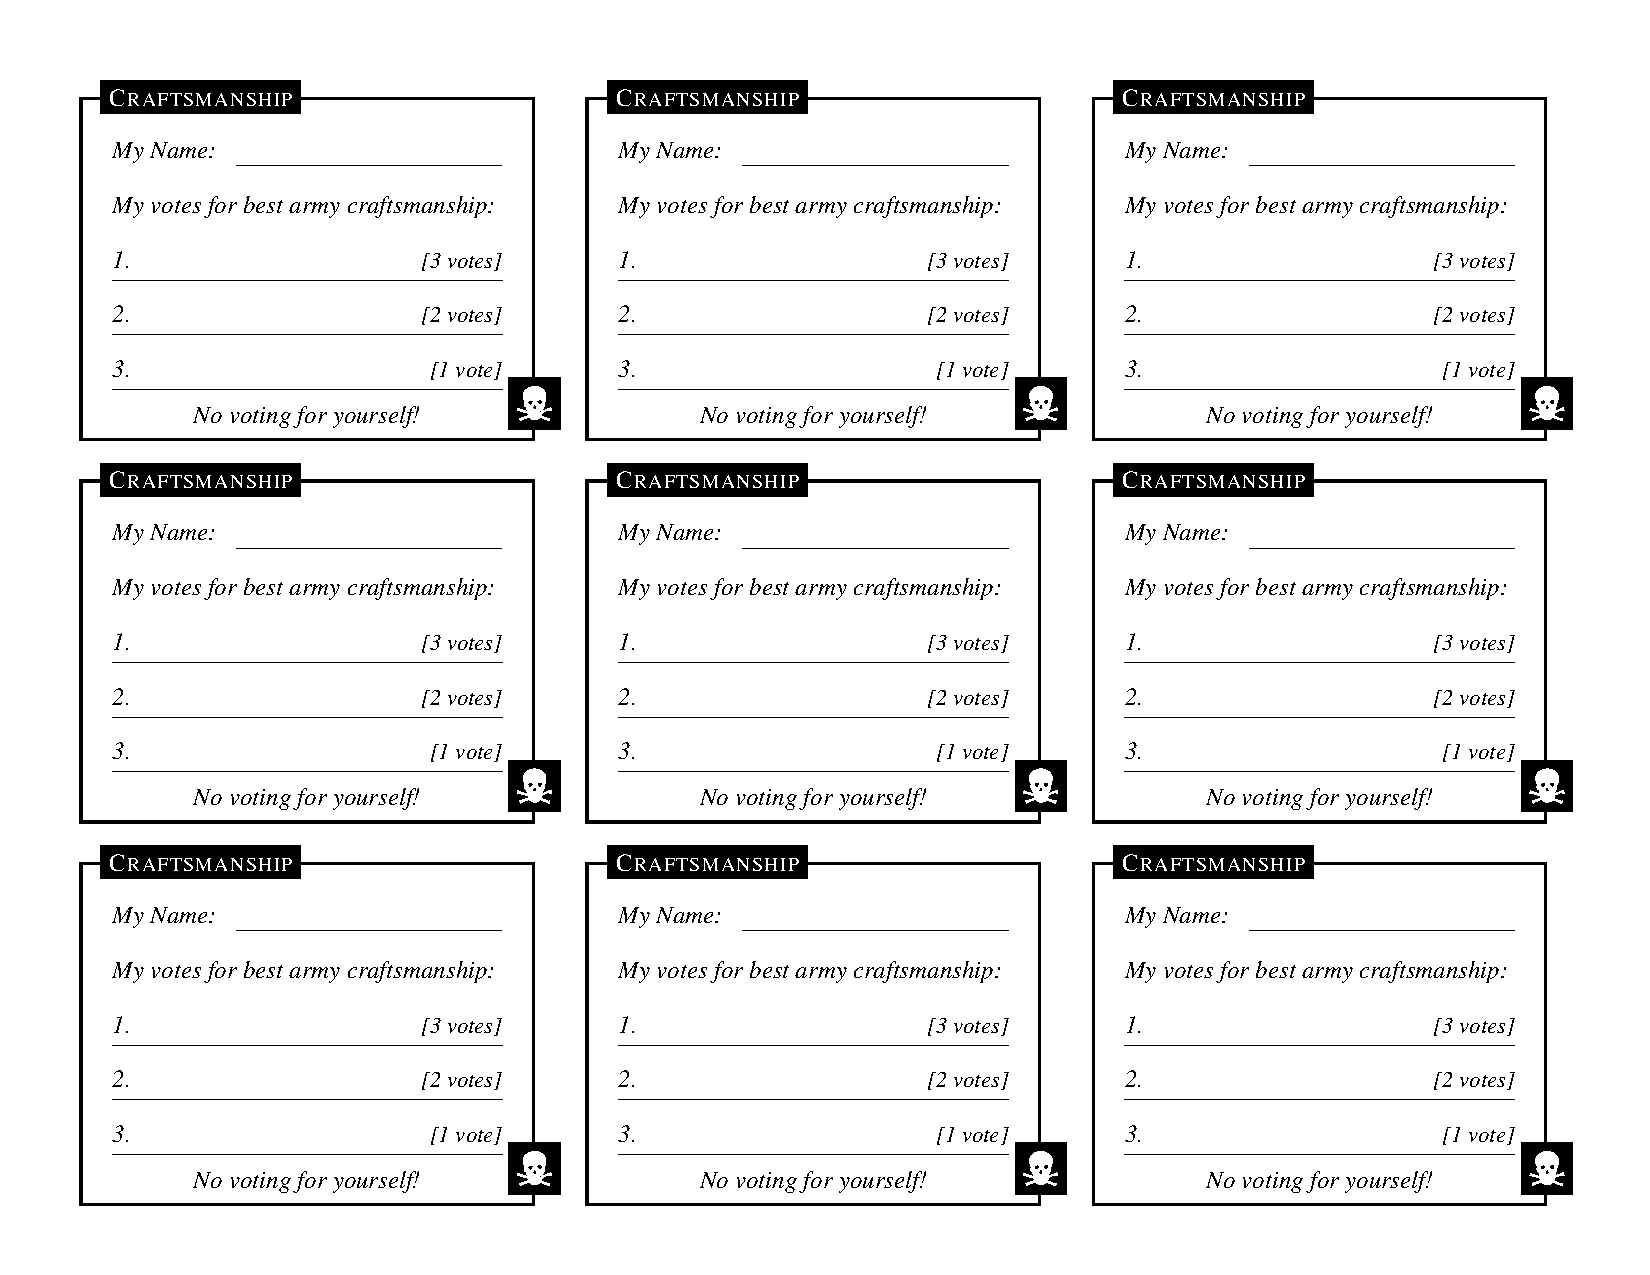
\includepdf[pages={1},landscape=true]{2016-painting.pdf}
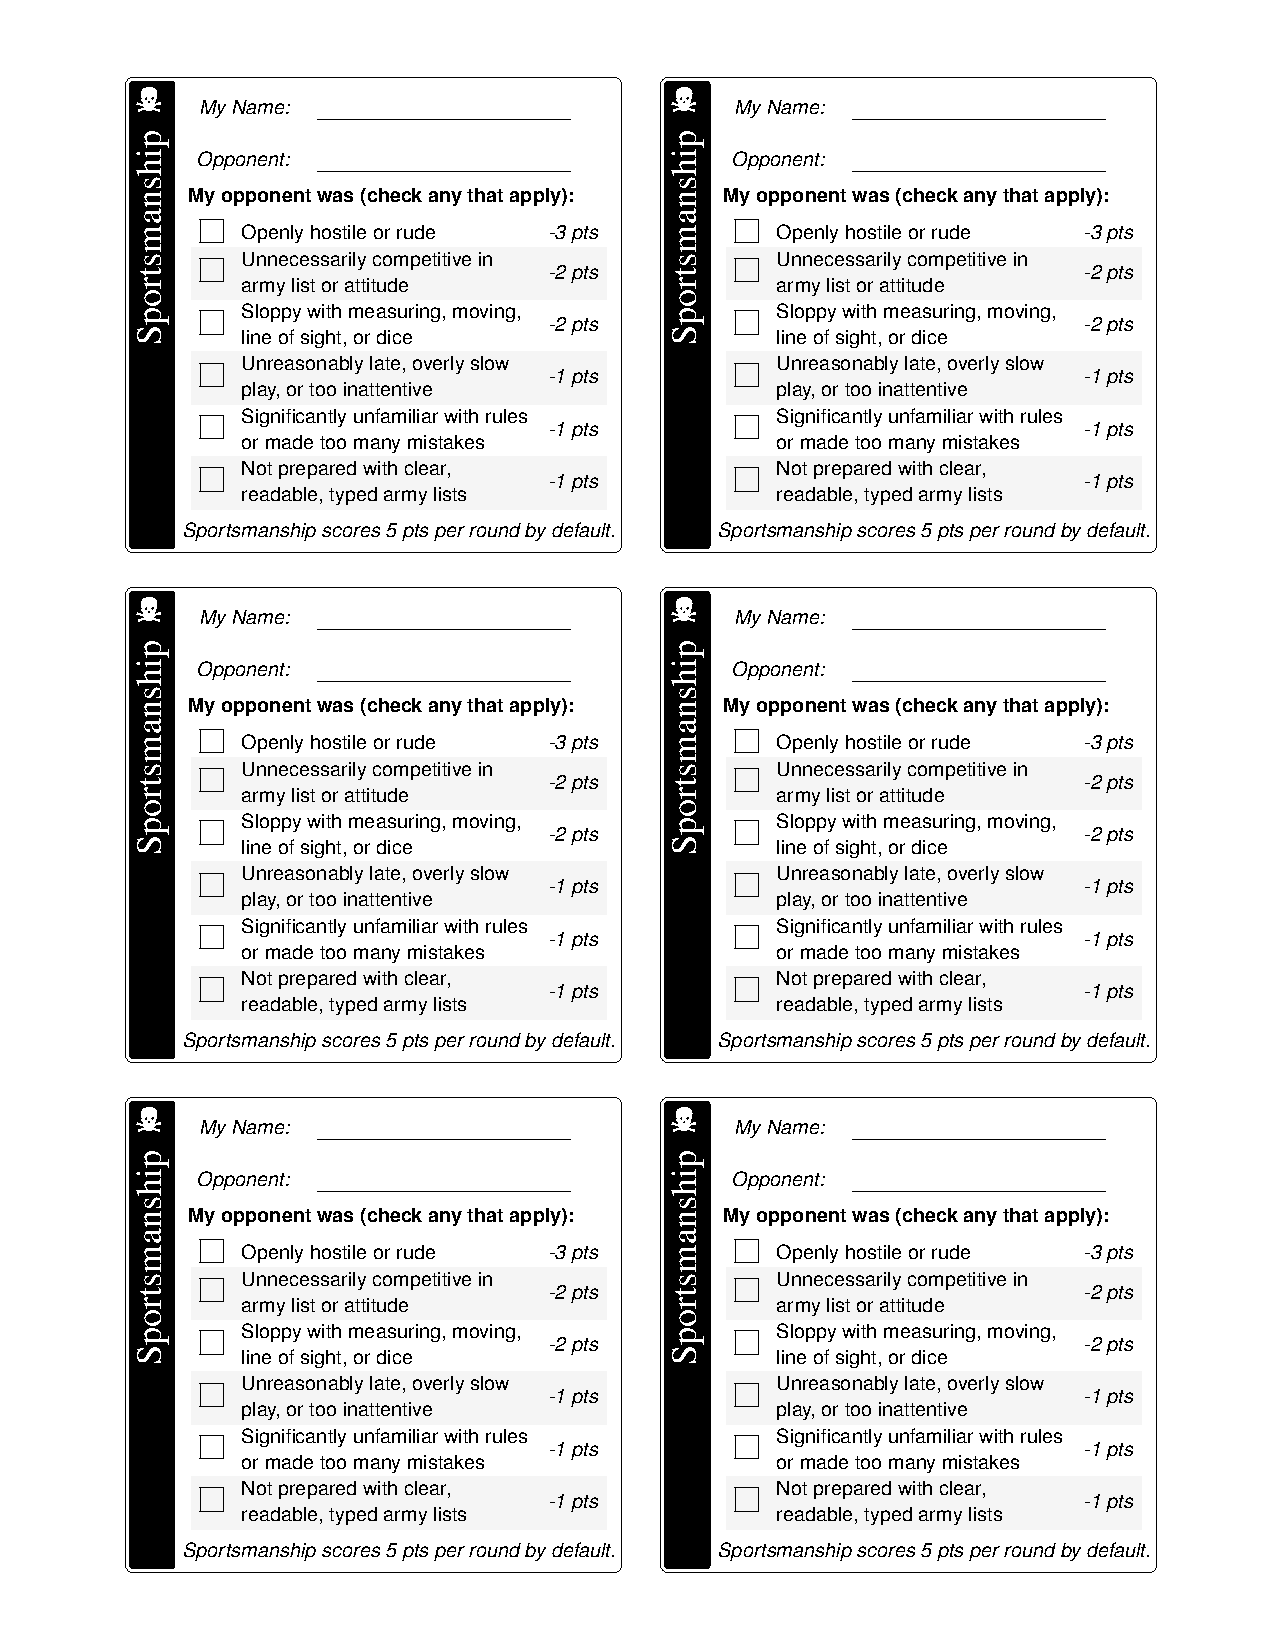
\includepdf[pages={1}]{2016-sportsmanship.pdf}
\restorebackground

%%----------------------------------------------------------------------
%%----------------------------------------------------------------------
\clearpage
\section{Missions}

\begin{columns}
  
  Army rules, legacies, and missions in this section should be read by
  all players.

\subsection{Campaign Framework}

The campaign consists of four rounds of Recon Squad skirmish matches,
followed by the Cataclysm, a climactic team battle.
The Recon Squad rules are available here:

\smallskip
\centerline{\url{rocketshipgames.com/40k/recon-squad/}}

\smallskip%
The Cataclysm uses standard 40k gameplay, caveat rules for team play.

At the start of the campaign, players join an alliance and choose a
legacy.  Legacies cannot be repeated within an alliance until all have
been chosen.  In each Recon Squad round the alliances alternate
choosing missions from this section.  Players that win at least two of
their legacy's three Recon Squad Missions in the listed roles of
attacker, defender, or either receive their legacy bonus in the
Cataclysm.

\subsection{Army Construction}

Each player must prepare two lists:

\begin{squishitemize}
  \item {Recon Squad:} For the skirmishes;
  \item {Cataclysm:} For the climactic finale.
\end{squishitemize}

Recon Squad lists are selected to at most~200 points, following the
rules in that packet.  Cataclysm lists are selected to at most~500
points by these rules:

  \begin{squishitemize}
  \item Each player's Recon Squad Detachment must be in their
    Cataclysm list.

  \item Additional units and models may be added to the Recon Squad
    Detachment.  The original models may not receive new wargear or
    upgrades.

  \item A single Cataclysm Reinforcements Detachment may be added to
    the army, with a force organization of~0--1 HQ,~1--3 Troop,~0--1
    Elite,~0--1 Fast Attack,~0--1 Heavy Support, and~0--1
    Fortification.  All its units must be chosen from a single
    faction, but that may be a different faction from the Recon Squad
    Detachment.

  \item No models are permitted that have more than~6 wounds.

  \item No models may have both a~2+ Armor and a~3+ Invulnerable save.

  \item No models or wargear are permitted that are restricted to a
    single instance (e.g., named characters).
  \end{squishitemize}

\end{columns}

%%----------------------------------------------------------------------
%%----------------------------------------------------------------------

%\vspace{-4pt}
\noindent
\begin{minipage}[t]{1.0\linewidth}\centering%
\rowcolors{2}{gray!12}{white}\setlength{\tabcolsep}{3pt}%
\resizebox{\linewidth}{!}{\begin{tabular}{|l|C{1in}|C{1in}|C{1in}|C{1in}|C{1in}|C{1in}|C{1in}|C{1in}|}
\hline
\rowcolor{gray!25} {\bf Mission}       
                    & {\bf Bodyguards}  & {\bf Excavators}& {\bf Headhunters}   & {\bf Killers}   & {\bf Penetrators}&{\bf Scouts}   & {\bf Sentinels} & {\bf Warriors}\\
\hline
\hline
{\bf Ambush}        & Defender          & Either         & Attacker             &                 &                 & Attacker       &                 &               \\
{\bf Assassination} & Defender          &                & Attacker             &                 & Attacker        &                &                 &               \\
{\bf Battlefield}   &                   &                &                      & Either          &                 &                &                 & Either        \\
{\bf Breakthrough}  & Attacker          &                &                      &                 & Attacker        &                & Defender        &               \\
{\bf Encirclement}  &                   &                &                      & Attacker        &                 &                & Defender        & Defender      \\
{\bf Excavation}    &                   & Either         & Either               &                 &                 & Either         &                 &               \\
{\bf Installation}  &                   & Either         &                      &                 & Attacker        &                & Defender        &               \\
{\bf Skirmish}      &                   &                &                      & Either          &                 & Either         &                 & Either        \\
\hline
\end{tabular}}

\small\it\smallskip
Recon Squad mission and role requirements for the legacies.
\end{minipage}

\clearpage
\squelchbackground

\noindent%
\legacycard{BODYGUARDS}%
{Our lives for you, my liege.\\~}%
{Ambush}%
{Defender}%
{Assassination}%
{Defender}%
{Breakthrough}%
{Attacker}%
{After all deployment, publicly pledge to one of your alliance's
  warlords other than your own.  You succeed if that warlord is in
  play at game end.}%
{Your pledged warlord gains a~5+ Invincible save.  When attached to
  one of your units it always passes Look Out, Sir rolls and your
  attached unit has Counter-Attack and Fearless.}
%%
\hfill
%%
\legacycard{EXCAVATORS}%
{Get it into the crates,\\quickly, this is ours!}%
{Ambush}%
{Either}%
{Excavation}%
{Either}%
{Installation}%
{Either}%
{After all deployment ends, secretly select an objective marker wholly
  outside your deployment zone.  You succeed if you control it at game
  end.}%
{Any non-vehicle or walker model of yours that starts the movement
  phase in contact with \emph{any} marker may move it up to 6'' with
  the model's movement.  The marker cannot leave the table or embark.}


\vfill

\noindent%
\legacycard{HEADHUNTERS}%
{Death comes for us all.\\We come for you.}%
{Ambush}%
{Attacker}%
{Assassination}%
{Attacker}%
{Excavation}%
{Either}%
{After all deployment, secretly select one of the opposing warlords.
  You succeed if that warlord is removed as a casualty by game end.}%
{All of your non-vehicle and walker models are considered to have
  Preferred Enemy, Precision Shot, and Precision Strike when attacking
  the selected warlord or an attached unit.}
%%
\hfill
%%
\legacycard{KILLERS}%
{Kill.  Maim.  Burn.\\~}%
{Battlefield}%
{Either}%
{Encirclement}%
{Attacker}%
{Skirmish}%
{Either}%
{After all deployment, publicly declare a crusade against an opposing
  player.  You succeed at game end if at most 25\% of that player's
  starting army points remain in play.}%
{All of your non-vehicle and walker models have Hatred and Fear when
  attacking that opponent's models.}


\pagebreak

\noindent%
\legacycard{PENETRATORS}%
{Everything has a weak spot.\\~}%
{Assassination}%
{Attacker}%
{Breakthrough}%
{Attacker}%
{Installation}%
{Attacker}%
{At game end your units control at least one primary objective marker
  in the opposing deployment zone.}%
{After all deployment you may ruin a piece of terrain or an opposing
  fortification, degrading any associated cover saves by~1 to a~6+
  at worst.  All of your non-vehicle and walker models gain Tank
  Hunter.}
%%
\hfill
%%
\legacycard{SCOUTS}%
{Let's go, on the move!\\~}%
{Ambush}%
{Attacker}%
{Excavation}%
{Either}%
{Skirmish}%
{Either}%
{Over the course of the game---not necessarily
  simultaneously---control at least three different objective
  markers outside your deployment zone at the end of any of your turns
  except Turn~1.}%
% {At the end of each of your turns except the first, make a note for
%   each primary objective marker you control outside your deployment
%   zone which you have not previously controlled.  You succeed if you
%   note at least three.}%
%
{Your non-vehicle models gain Crusader, Move Through Cover, and
  Infiltrate.}

\vfill


\noindent%
\legacycard{SENTINELS}%
{None shall pass.\\~}%
{Breakthrough}%
{Defender}%
{Encirclement}%
{Defender}%
{Installation}%
{Defender}%
{At game end your units control all the primary objective markers that
  began in your deployment zone.}%
{After all deployment you may bolster a piece of terrain or a
  fortification in your deployment zone, improving any associated
  cover save by~1 to a~2+ at best.  All of your non-vehicle and walker
  models gain Stubborn.}
%%
\hfill
%%
\legacycard{WARRIORS}%
{This isn't over.\\This will never be over.}%
{Battlefield}%
{Either}%
{Encirclement}%
{Defender}%
{Skirmish}%
{Either}%
{There are no enemy models in your deployment zone at
  game end.}%
{All of your non-vehicle and walker models gain Feel No Pain (6+) and
  your vehicles gain It Will Not Die.}


\clearpage
\restorebackground


\newcommand{\scoringbox}[5]{%
\vfill%
\vspace{9pt}%
\noindent\vbox{%
\noindent\vbox to -4pt{\noindent\hfill\Large\bf\sc\fontfamily{ptm}\selectfont Scoring\vbox{}}\\
%
{\fbox{\vbox{\small%
\setlength{\tabcolsep}{2pt}%
\noindent\begin{tabularx}{\linewidth}{cccX}
  \hbox to 1.25em{\rotatebox{45}{\small\bf Attacker}}&
  \hbox to 1.25em{\rotatebox{45}{\small\bf Defender}}&
  &
  \multicolumn{1}{c}{\footnotesize\bf Condition}
\\
  \hline
%
  \rescheck&\rescheck& & {\bf Major Victory:} #1\\
%
  \rescheck&\rescheck& &
  {\bf Minor Victory:} #2\\
%
\rescheck&\rescheck& &
{\bf Draw:} #3\\
\hline \rescheck&\rescheck& &
{\bf Bonus Point:} #4\\
\rescheck&\rescheck& &
{\bf Bonus Point:} #5\\
\end{tabularx}%
}}}}%
}

\clearpage
\squelchbackground

%%----------------------------------------------------------------------
%%----------------------------------------------------------------------
\clearpage
\section{Mission: Ambush}

%\begin{columns}
A supply convoy is moving through the area!
\begin{squishitemize}
\item{\bf Attacker:} You \emph{need} those supplies.
\item{\bf Defender:} The supplies must get through.
\end{squishitemize}

\subsection{\bf The Battlefield}%

The winner of the deployment zone roll off chooses a table edge and
the other player takes the opposite.  The defender's deployment zone
is the~12'' strip along their table edge.  The attacker's deployment
zone is the 6'' strips along both side edges of the battlefield, up to
9'' away from the defender's deployment zone.

\subsection{\bf Mission Rules}%

%The attacker plays first.  The defender may not Seize the Initiative.

At the start of their deployment, the defender gains a Bulldog convoy
vehicle for their army:

\vspace*{-9pt}
  \begin{center}
  \begin{tabular}[t]{O{1.5in}cccccccccE{1.5in}}
    & {\bf M} & {\bf WS} &  {\bf BS} & {\bf S} & {\bf T} & {\bf W} & {\bf A} & {\bf Ld} & {\bf Sv} & {\bf Keywords}\\
    \hline
    {\bf Bulldog} & 12'' & - & - & 6 & 7 & 12 & - & - & 3+ & Vehicle\\
  \end{tabular}
  \end{center}

\vspace*{-9pt}
  \hfill
  \begin{minipage}{6in}
  \noindent\textbf{Smoke Launchers (4).} Up to four times per game, the
  Bulldog may use its smoke launchers in your shooting phase.  If you
  do so, your opponent must subtract~1 from all hit rolls against this
  model from shooting attacks until your next turn.

  \noindent\textbf{Advanced Repair Systems.}  Roll a D6 at the start of each
  of your turns; on a 6 the Bulldog regains up to two lost wounds.

  \noindent\textbf{On Assignment.}  The Bulldog is taken to have
  whatever faction keywords are shared by all of the units in your
  army list (all of the partners' lists in team games).

%  \noindent\textbf{Convoy.}
  \end{minipage}
  \hfill\hbox to 0pt{}

  \vfill

  If destroyed, leave the wrecked Bulldog model in place.  The
  Bulldog, or its wreck, act as an objective marker.  While not
  destroyed the defender controls it by default if there are no
  attacker models within 3''.


  \scoringbox%
  {Attacker if the Bulldog is destroyed and they control its wreck.
    Defender if the Bulldog or its wreck is within 12'' of the
    attacker table edge and they control it.}%
  {Attacker if the Bulldog is not destroyed but they control it.
    Defender if they control the Bulldog or its wreck, but it is not
    within 12'' of the attacker table edge.}%
  {The Bulldog or its wreck is contested.}%
  {Opponent's leader is a casualty.}%
  {Player's leader survives.}

%\end{columns}

%%----------------------------------------------------------------------
%%----------------------------------------------------------------------
\clearpage
\section{Mission: Assassination}

  A VIP is touring the frontlines, their mission unknown.
  \begin{squishitemize}
  \item {\bf Attacker:} The VIP must be slain.
  \item {\bf Defender:} The VIP must be defended at all cost.
  \end{squishitemize}

\subsection{\bf The Battlefield}%

Deployment zones are 12'' from opposing table edges.  Place~3
objective markers at~12'' intervals along the centerline 24'' from
both player table edges.

\subsection{\bf Mission Rules}%

At the start of their deployment, the defender gains a VIP for their army:

\vspace*{-9pt}
\begin{center}    
  \begin{tabular}[t]{O{1.5in}cccccccccE{2.5in}}
    & {\bf M} & {\bf WS} & {\bf BS} & {\bf S} & {\bf T} & {\bf W} & {\bf A} & {\bf Ld} & {\bf Sv} & {\bf Keywords}\\
\hline
    {\bf VIP} & 6 & 4+ & 4+ & 3 & 3 & 6 & 2 & 10 & 4+ & Character, Infantry\\
  \end{tabular}
  \end{center}

  \vspace*{-9pt}
  \hfill
  \begin{minipage}{6in}
    \noindent\textbf{Refractor Field.} This model has a~5+ invulnerable
    save.

    \noindent\textbf{On Assignment.}  This unit is taken to have whatever
    faction keywords are shared by all of the units in your army list
    (all of the partners' lists in team games).
  \end{minipage}
  \hfill\hbox to 0pt{}

  At game end, each objective marker is worth~1 victory point.  The
  defender gets~2 victory points for each wound remaining on the VIP.
  The attacker gets~2 victory points for each wound lost by the VIP.

\vfill  
\scoringbox%
{Player has at least twice as many victory points as their opponent.}%
{Player has more victory points.}%
{Players have equial victory points.}%
{Opponent's leader is a casualty.}%
{Player has a model in opponent's deployment zone.}



%%----------------------------------------------------------------------
%%----------------------------------------------------------------------
\clearpage
\section{Mission: Battlefield}


The war grinds on interminably, all notion of battle lines lost in
confusion and exhaustion.

\begin{squishitemize}
\item \textbf{Attacker} and \textbf{Defender} roles are identical in
  this mission and have no effect in-game.
\end{squishitemize}

\subsection{\bf The Battlefield}%

The winner of a~D6 roll off chooses a table corner.  Their deployment
zone is the quarter circles of all points within~12'' of that corner
as well as the \emph{diagonally} opposite corner.  The other player's
deployment zone is the~12'' quarter circles from the other corners.

Place a single objective marker at table center.

% \vfill
% \vbox to 0pt{}
% \columnbreak

\subsection{\bf Mission Rules}%

At game end, victory points are earned as follows:

\begin{squishitemize}
\item At least~3 of your opponent's models have been removed as
  casualties: +2

\item At least 50\% of your opponent's army by points or models are
  casualties: +3

\item The total number of wounds lost by your opponent is more than
  you: +1

\item All of your opponent's models have been removed as casualties:
  +1
\end{squishitemize}

\vfill

\scoringbox%
{Player has at least twice as many victory points as their opponent.}%
{Player has more victory points.}%
{Players have equial victory points.}%
{Opponent's leader is a casualty.}%
{Controls the objective marker.}

%%----------------------------------------------------------------------
%%----------------------------------------------------------------------
\clearpage
\section{Mission: Breakthrough}

  Opposing forces thrust and counter-thrust to break up or hold
  battlefield positions.
  \begin{squishitemize}
  \item {\bf Attacker:} You must pierce the enemy's lines.
  \item {\bf Defender:} Hold your ground.
  \end{squishitemize}

\subsection{\bf The Battlefield}%

Deployment zones are~12'' from opposing table edges.

\subsection{\bf Mission Rules}%

At game end, victory points are earned as follows:

\begin{squishitemize}
\item The defender earns~2 victory points for each quarter of their
  army by number of models that has not been removed as a casualty,
  rounding down (i.e., less than~25\% is worth no points).

\item The defender earns~1 victory point if no enemy models are in
  their table half.

\item The attacker earns~1 victory point for each quarter of their
  army by models that has not been removed as a casualty, rounding
  down.

\item The attacker earns~1 victory point for each quarter of their
  starting army by models that is at least partially within 6'' of the
  defender table edge, rounding up (i.e., having at least~1 model
  within 6'' of the defender edge is worth a point).

\end{squishitemize}

% \vfill
% \vbox to 0pt{}
% \columnbreak

\vfill
\scoringbox%
{Player has at least twice as many victory points as their opponent.}%
{Player has more victory points.}%
{Players have equial victory points.}%
{Opponent's leader is a casualty.}%
{Leader is within 12'' of opponent's player table edge.}

% \scoringbox%
% {Attacker if they control at least~3 objective markers.  Defender if
% the attacker controls no objective markers.}%
% {Attacker if they control at least~1 objective marker.}%
% {Otherwise.}%
% {Opponent's leader is a casualty.}%
% {Player's leader is the closest model to the defender's table edge.}

% \scoringbox%
% {Attacker if at least~50\% of their starting army by number of models
%   is at least partially within~6'' of the defender's table edge.
%   Defender if attacker has no models within~6'' of the defender's
%   table edge.}%
% {Attacker if more than~25\% of their starting army by number of models
%   is at least partially within~6'' of the defender's table edge.
%   Defender if attacker has at most 25\% of their starting army by
%   points value or number of models within~6'' of the defender's table
%   edge.}%
% {Otherwise.}%
% {Opponent's leader is a casualty.}%
% {Player's leader is the closest model to the defender's table edge.}

%%----------------------------------------------------------------------
%%----------------------------------------------------------------------
\clearpage
\section{Mission: Encirclement}

  A small force has been outmaneuvered and surrounded in a tight
  pocket of the battle.

  \begin{squishitemize}
  \item {\bf Attacker:} Crush them.
  \item {\bf Defender:} Survive.
  \end{squishitemize}

\subsection{\bf The Battlefield}%

The winner of a~D6 roll off chooses a table edge and the other player
takes the opposite.  The attacker's deployment zone is~6'' from
\emph{both} player table edges.  The defender's deployment zone is
the~12'' center strip~18'' from both player table edges.


\subsection{\bf Mission Rules}%

At game end, victory points are earned as follows:

\begin{squishitemize}
\item At least~3 of your opponent's models have been removed as
  casualties: +2

\item At least 50\% of your opponent's army by points or models are
  casualties: +3

\item The total number of wounds lost by your opponent is more than
  you: +1

\item All of your opponent's models have been removed as casualties:
  +1
\end{squishitemize}

\vfill

\scoringbox%
{Player has at least twice as many victory points as their opponent.}%
{Player has more victory points.x}%
{Players have equial victory points.}%
{Opponent's leader is a casualty.}%
{Player has a model in each table quadrant, at least~3'' from table center.}


%%----------------------------------------------------------------------
%%----------------------------------------------------------------------
\missiontitle{Mission: Excavation}

\begin{columns}

  An important relic was uncovered by an excavation team just before
  they were forced to abandon the site by the encroaching battle.  It
  must be retrieved!

  \textbf{Attacker} and \textbf{Defender} roles are identical in this
  mission and have no effect in-game.

\missionheading{The Battlefield}%

Deployment zones are 12'' from opposing table edges.  The winner of
a~D6 roll off chooses a side and the other player takes the opposite.

Place a primary objective marker at the center of the table and
secondary objective markers at the center of each table quadrant.


\missionheading{Mission Rules}%

Any model that starts the movement phase in base to base contact with
the \emph{primary} objective marker while no enemy models are in base
to base contact with it may move the marker with itself up to a total
of 6'' in the movement phase, ending in contact with the model.  The
marker cannot leave the table or embark.

%\columnbreak

At game end, control of the primary objective is worth~3 victory
points while each secondary objective is worth~1 victory point.

\scoringbox%
{Player controls the primary objective and has more victory points.}%
{Player has more victory points.}%
{Players have equal victory points.}%
{Opponent's leader is a casualty.}%
{The primary objective marker is fully within your deployment zone.}

\end{columns}

%%----------------------------------------------------------------------
%%----------------------------------------------------------------------
\missiontitle{Mission: Installation}

\begin{columns}

  A critical bunker outpost, command center, supply warehouse, or
  temple has come under siege!

{\bf Attacker:} You must seize control of the site.

{\bf Defender:} You must protect the site.

\missionheading{The Battlefield}%

Deployment zones are 12'' from opposing table edges, with the attacker
choosing and the defender taking the opposite.  Place a small
building, roughly~6''x6''x3'', centered 12'' from the defender's table
edge.  The defender may deploy units embarked in the building or on
the battlements.

\missionheading{Mission Rules}%

The defender deploys first but the attacker chooses to play first or
second after all deployment concludes.  Seize the Initiative applies.

Control of the building or its ruins is determined as an objective
marker, including embarked models.

The building has armor~11 on each facing,~2 hull points, a capacity
of~5, and battlements on top.

\columnbreak

\scoringbox%
{Player controls the building/ruins.}%
{Attacker if the building is ruined and contested; defender if the
  building is not ruined but is contested.}%
{Neither player contests or holds the building or its ruins.}%
{Opponent's leader is a casualty.}%
{Opponent has less than 25\% of their starting army remaining, by
  points value or number of models.}

\end{columns}

%%----------------------------------------------------------------------
%%----------------------------------------------------------------------
\missiontitle*{Mission: Skirmish}

\begin{columns}

  Vanguards patrolling the outskirts of their main forces have crashed
  into each other---contact is made!

  \textbf{Attacker} and \textbf{Defender} roles are identical in this
  mission and have no effect in-game.

\missionheading{The Battlefield}%

% A variety of ruins, woods, and other terrain should be placed to
% cover a quarter to a half of the board evenly and roughly
% symmetrically.

Deployment zones are diagonal table corners, up to~12'' from the
centerline between them.  Roll off to determine who chooses a corner
and their player table edge, the other player taking the opposite.

Place objective markers at the center of the table and the centers of
the two table quadrants opposite the deployment zone corners.

\columnbreak

\scoringbox%
{Player controls at least two more objective markers than opponent, or
  opponent has been completely eliminated.}%
{Player controls at least one more objective marker than opponent.}%
{Players control equal objective markers.}%
{Opponent's leader is a casualty.}%
{Player has at least one model within 12'' of at least two table
  corners, not including their deployment corner.}

\end{columns}
%

\clearpage
\restorebackground


%%%----------------------------------------------------------------------
%%----------------------------------------------------------------------
\section{The Cataclysm}

\begin{columns}
  
  All of the recon squads have crossed paths as they fight toward
  their final missions!

  The alliance with fewer total points earned in the Recon Squad
  matches is the {\bf Defender}, and the other the {\bf Attacker}.

  \subsection{Heroes}

  Each Recon Squad's specialists that are not already Characters are
  elevated to such and improve their wounds characteristics by~1,
  except the leader, which improves their wounds characteristic by~2.
  The leader is considered an HQ unit as well as their original
  battlefield role, and must be their player's warlord, gaining a
  trait as usual.  Before any deployment begins both alliances
  simultaneously declare one of their warlords to be their warmaster.

  \subsection{The Battlefield}

  Deployment zones are the areas up to~12'' from the long edges of the
  battlefield (Dawn of War).  The defender chooses a zone and the
  attacker takes the other.  Beginning with the defender, the
  alliances alternate placing primary objective markers in their own
  deployment zones up to~3 each, for a total of~6 on the battlefield.
  Beginning with a defender and alternating between the alliances,
  each player then places a secondary objective marker outside their
  deployment zone.

  Deployment begins with the defender and proceeds as usual for
  Matched Play.

  \subsection{Endgame}

  The Cataclysm ends after battle round~5.

  \subsection{Scoring}

  Objective markers are scored after each game turn: Primaries award
  the current turn number in victory points, while secondaries award~1
  victory point.

  % \begin{itemize}
  % \item Primaries award the current turn number in victory points;
  % \item Secondaries award~1 victory point.
  % \end{itemize}

  Alliances gain~2 victory points if the opposing warmaster is removed
  as a casualty, and~1 victory point for each other opposing warlord
  eliminated.

  First Blood and Linebreaker both apply as in the standard Eternal
  War missions.

  % The first unit (including single models) to be removed in its
  % entirety for any reason yields~1 victory point to the opposing
  % alliance for first blood.  If an alliance has any scoring units in
  % its opponent's deployment zone at game end then it scores~1 victory
  % point for linebreaker.

  Whichever alliance scores the most victory points wins a tactical
  victory in the Cataclysm, while the alliance that has more players
  achieve their legacy objectives wins a strategic victory.

\end{columns}


\end{document}

\missionheading{Disclaimer}%

Cataclysm is completely unofficial, unauthorized, and unaffiliated
with Games Workshop.

\smallskip%
{\small Adepta Sororitas, Adeptus Astartes, Astra Militarum, Blood
  Angels, Chaos Daemons, Chaos Space Marines, Dark Angels, Dark Eldar,
  Eldar, Grey Knights, Militarum Tempestus, Necrons, Officio
  Assassinorum, Space Wolves, Tau Empire, Tyranid, Forge World, Games
  Workshop, Warhammer, and all associated marks, names, races, race
  insignia, characters, vehicles, locations, units, illustrations,
  images, and models from the Warhammer~40,000 universe and game are
  either \textregistered, TM, and/or \textcopyright\ Copyright Games
  Workshop Ltd~2000--2014, variably registered in the UK and other
  countries.  Used without permission, no challenge to status
  intended, all rights reserved to their respective owners.}


